\chapter{Experimental Results}
\label{ch:experiments}

This chapter reports quantitative and qualitative results on the 15-scene benchmark. Experiments use grid-search overrides (\texttt{scene\_method\_overrides.json}) for routed mathematical outputs, optional TinyResidualRefiner refinement (\texttt{student\_runK.pt}), and DeepFilterNet3 teacher references. All RMS errors are computed against \texttt{clean\_reference.wav} with sample-aligned waveforms.

\section{Experimental Setup}
\label{sec:exp_setup}

\subsection{Implementation Details}

\begin{table}[H]
  \centering
  \caption{Implementation environment for reported results.}
  \label{tab:exp_impl}
  \begin{tabular}{ll}
    \toprule
    \textbf{Component} & \textbf{Version / setting} \\
    \midrule
    Python               & 3.13 (Docker images use 3.11-slim) \\
    NumPy / SciPy        & 2.4 / 1.17 \\
    PyTorch              & 2.11+cpu \\
    STFT                 & $N_{\mathrm{FFT}}=512$, hop 128, Hann \\
    Student checkpoint   & \texttt{student\_runK.pt} ($\alpha=0.8$, 56\,129 params) \\
    Teacher              & DeepFilterNet3 (\texttt{models/DeepFilterNet3/}, dfnet311 CLI) \\
    Routed outputs       & \texttt{run\_pipeline.py --all} + overrides \\
    \bottomrule
  \end{tabular}
\end{table}

Training \texttt{runK} consumed 21\,488 steps in 1200\,s on CPU (\texttt{train\_log\_runK.json}, val L1 $\approx 0.386$). Evaluation uses \texttt{eval\_runK.py} on \texttt{outputs/distill\_refined\_runK/}; results are exported to \texttt{distill\_eval.json}.

\subsection{Evaluation Protocol}

Three enhancement stages are compared: base OM-LSA/MCRA, routed math (override), and runK distill refined. DeepFilterNet3 teacher WAVs provide an offline upper bound. Primary metric: RMS error $e_{\mathrm{RMS}}$ against \texttt{clean\_reference.wav}. Secondary metrics include SNR (Table~\ref{tab:exp_snr_summary}) and web-platform prefix SNR for uploads (\chapref{ch:web}).

\section{Routing Configuration and Per-Scene Methods}
\label{sec:exp_routing}

Routed outputs use \texttt{scene\_method\_overrides.json}. Override routing improves mean RMS relative to base OM-LSA; per-scene module assignments are logged in \texttt{routed\_route\_log.json} (\chapref{ch:routing}).

\section{Distillation Refinement Results}
\label{sec:distill_results}

Table~\ref{tab:distill_full} reports \texttt{distill\_eval.json} (runK). Distillation improves routed RMS in \textbf{all 15 scenes} (mean $\Delta e=1.39\times10^{-3}$). Largest gains: scene11 (bursts, $\Delta=0.00569$), scene09 (chirp, $\Delta=0.00436$), scene02 (white 5\,dB, $\Delta=0.00102$).

\begin{table}[H]
  \centering
  \caption{Full distillation A/B results (\texttt{student\_runK.pt}, RMS vs.\ clean).}
  \label{tab:distill_full}
  \footnotesize
  \setlength{\tabcolsep}{3pt}
  \begin{tabular}{lrrrrr}
    \toprule
    \textbf{Scene} & $e_{\mathrm{base}}$ & $e_{\mathrm{routed}}$ & $e_{\mathrm{runK}}$ & $e_{\mathrm{teacher}}$ & $\Delta$ \\
    \midrule
    S01 white 15\,dB  & 0.00638 & 0.00623 & 0.00537 & 0.00441 & 0.00086 \\
    S02 white 5\,dB   & 0.01065 & 0.01003 & 0.00901 & 0.00766 & 0.00102 \\
    S03 pink 10\,dB   & 0.00807 & 0.00808 & 0.00698 & 0.00529 & 0.00110 \\
    S04 brown 8\,dB   & 0.00595 & 0.00555 & 0.00485 & 0.01076 & 0.00069 \\
    S05 hum50         & 0.00620 & 0.00538 & 0.00471 & 0.00340 & 0.00067 \\
    S06 hum60         & 0.00652 & 0.00554 & 0.00494 & 0.00347 & 0.00060 \\
    S07 HF hiss       & 0.00659 & 0.00655 & 0.00562 & 0.00406 & 0.00093 \\
    S08 LF rumble     & 0.00710 & 0.00673 & 0.00575 & 0.00435 & 0.00099 \\
    S09 chirp         & 0.01506 & 0.01686 & 0.01249 & 0.00447 & 0.00436 \\
    S10 clicks        & 0.01062 & 0.00845 & 0.00754 & 0.00626 & 0.00091 \\
    S11 bursts        & 0.01596 & 0.01412 & 0.00842 & 0.00655 & 0.00569 \\
    S12 babble        & 0.01458 & 0.01379 & 0.01284 & 0.01080 & 0.00095 \\
    S13 street        & 0.01001 & 0.00932 & 0.00831 & 0.00727 & 0.00101 \\
    S14 office fan    & 0.00945 & 0.00785 & 0.00765 & 0.00578 & 0.00020 \\
    S15 reverb+hiss   & 0.00728 & 0.00724 & 0.00644 & 0.00476 & 0.00081 \\
    \midrule
    \textbf{Mean}     & 0.00936 & 0.00837 & 0.00730 & 0.00596 & 0.00139 \\
    \bottomrule
  \end{tabular}
\end{table}

\begin{table}[H]
  \centering
  \caption{Aggregate RMS and SNR comparison across enhancement stages.}
  \label{tab:distill_summary}
  \begin{tabular}{lcc}
    \toprule
    \textbf{Stage} & \textbf{Mean $e_{\mathrm{RMS}}$} & \textbf{Scenes improved vs prev stage} \\
    \midrule
    Base OM-LSA only           & 0.00936 & --- \\
    Routed (override)          & 0.00837 & 13 / 15 vs base \\
    + runK distill refine      & 0.00730 & 15 / 15 vs routed \\
    DeepFilterNet3 teacher     & 0.00596 & 14 / 15 vs runK \\
    \bottomrule
  \end{tabular}
\end{table}

\begin{table}[H]
  \centering
  \caption{Mean SNR summary (dB, 15 scenes).}
  \label{tab:exp_snr_summary}
  \begin{tabular}{lcccc}
    \toprule
    & Noisy & Routed & runK & Teacher \\
    \midrule
    Mean SNR (dB) & 9.07 & 12.69 & 14.06 & 16.07 \\
    \bottomrule
  \end{tabular}
\end{table}

The runK student closes approximately 44\% of the gap between routed math and teacher in mean RMS, at $\sim\!350\times$ lower refine inference cost than DeepFilterNet3 (\chapref{ch:dl}).

\begin{figure}[H]
  \centering
  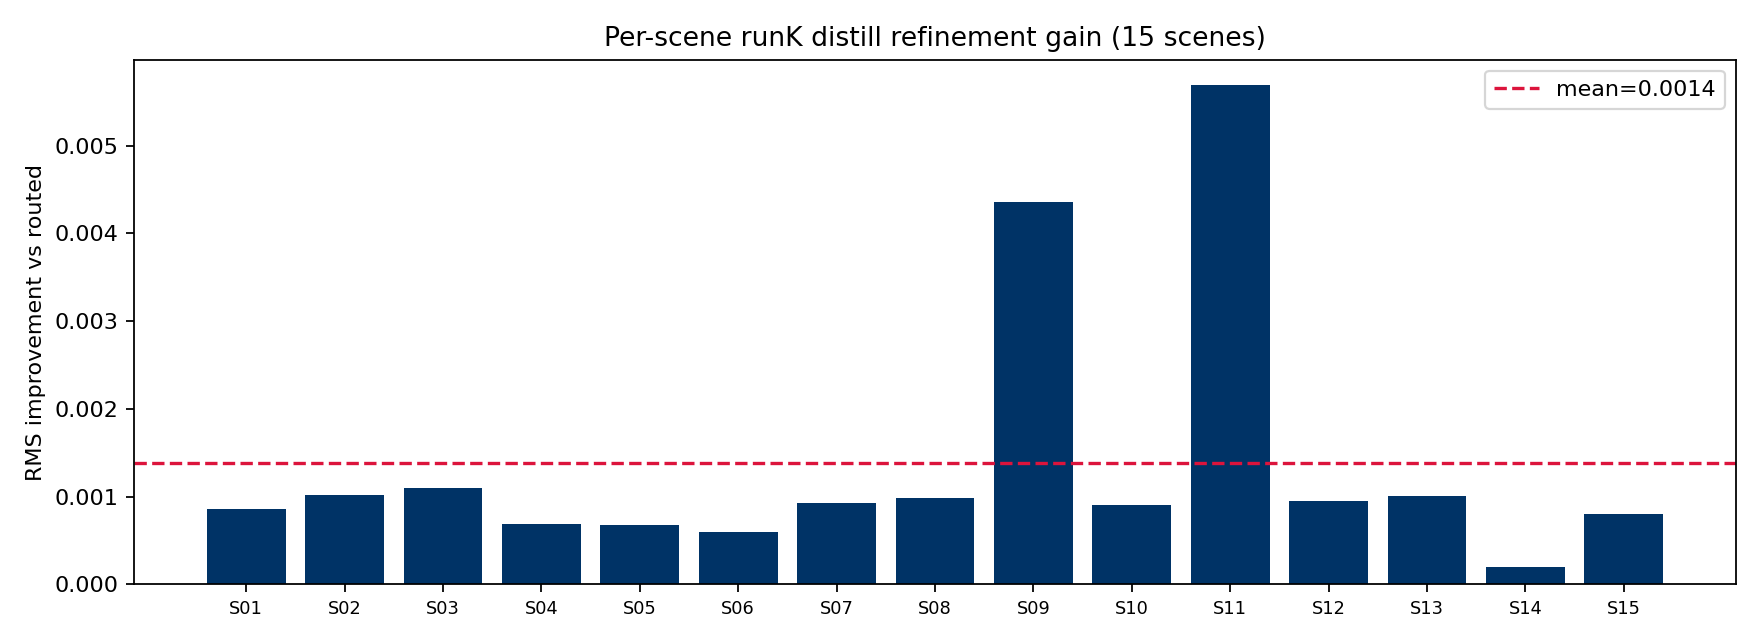
\includegraphics[width=0.92\textwidth]{figures/experiments/rms_improvement_bar.png}
  \caption{Per-scene RMS improvement from runK TinyResidualRefiner over routed outputs. Scene11 and S09 show the largest absolute gains.}
  \label{fig:rms_improvement_bar}
\end{figure}

\section{Routing Ablation}
\label{sec:routing_ablation}

Figure~\ref{fig:routing_ablation} summarizes ablation from monolithic OM-LSA to adaptive routing to runK hybrid distillation.

\begin{figure}[H]
  \centering
  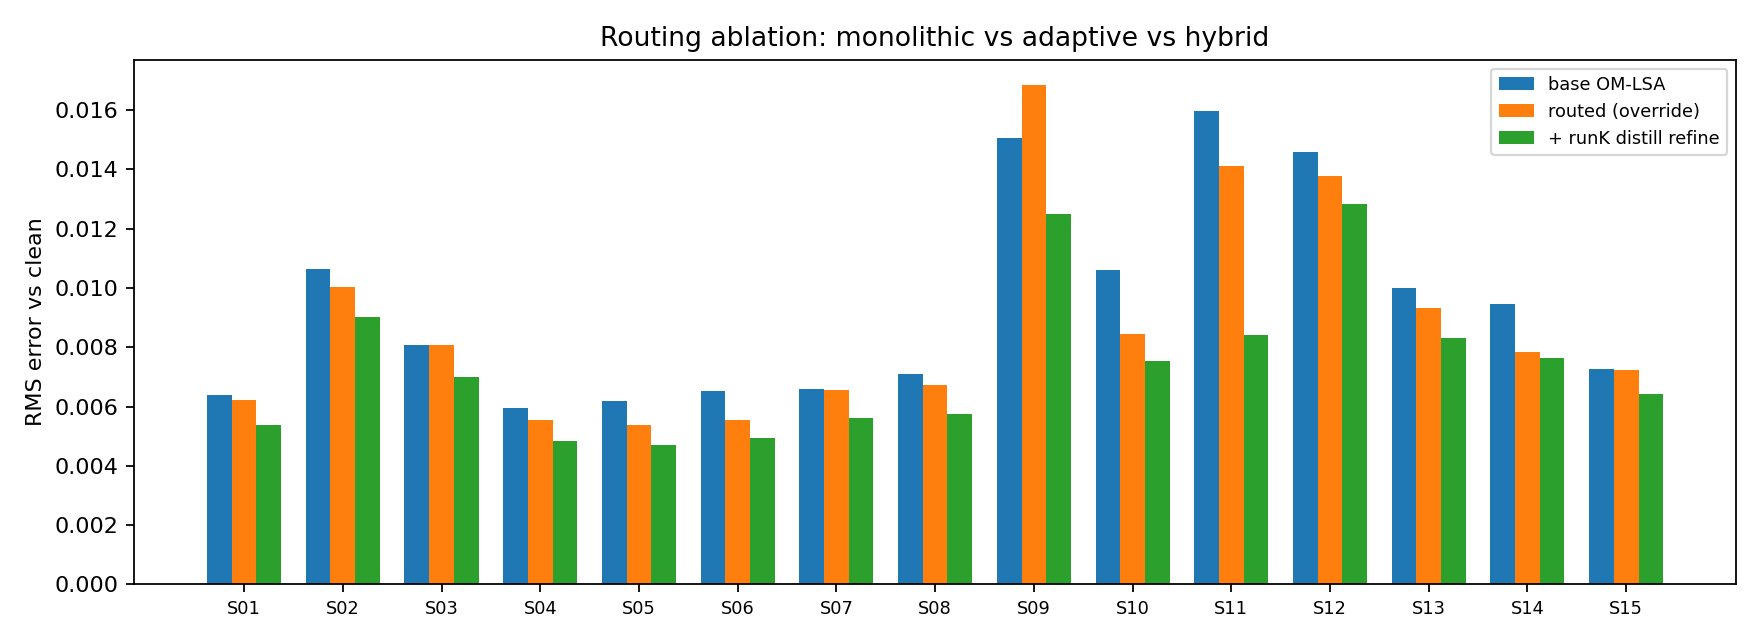
\includegraphics[width=0.92\textwidth]{figures/experiments/routing_ablation_rms.png}
  \caption{Routing ablation: base OM-LSA vs.\ routed vs.\ runK distill-refined RMS error per scene.}
  \label{fig:routing_ablation}
\end{figure}

On scene09, runK refinement reduces routed RMS from $0.01686$ to $0.01249$ ($-26\%$); on scene11, from $0.01412$ to $0.00842$ ($-40\%$).

\section{Qualitative Analysis}
\label{sec:qualitative}

Figures~\ref{fig:spectrogram_comparison}--\ref{fig:spec_scene15} compare noisy mixture, routed output, \textbf{runK refined} output, and clean reference (spectrograms regenerated from \texttt{distill\_refined\_runK/}).

\begin{figure}[H]
  \centering
  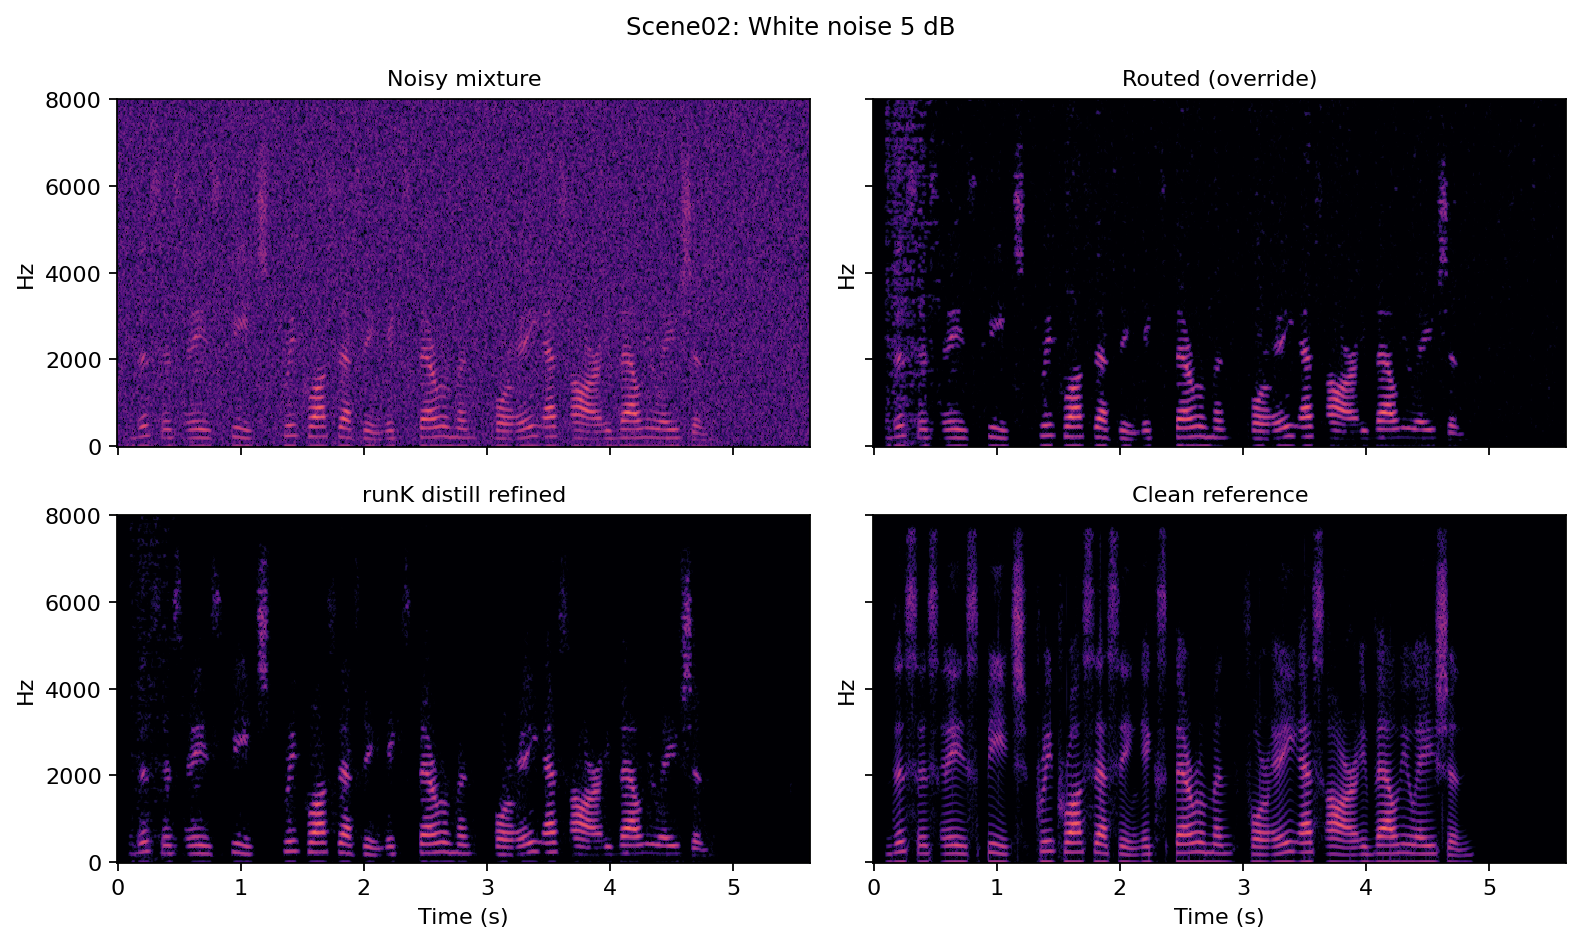
\includegraphics[width=0.95\textwidth]{figures/experiments/spectrogram_scene02_white_snr5.png}
  \caption{Scene02 (white noise, 5\,dB): runK refinement further sharpens harmonics after NMF routing.}
  \label{fig:spectrogram_comparison}
\end{figure}

\begin{figure}[H]
  \centering
  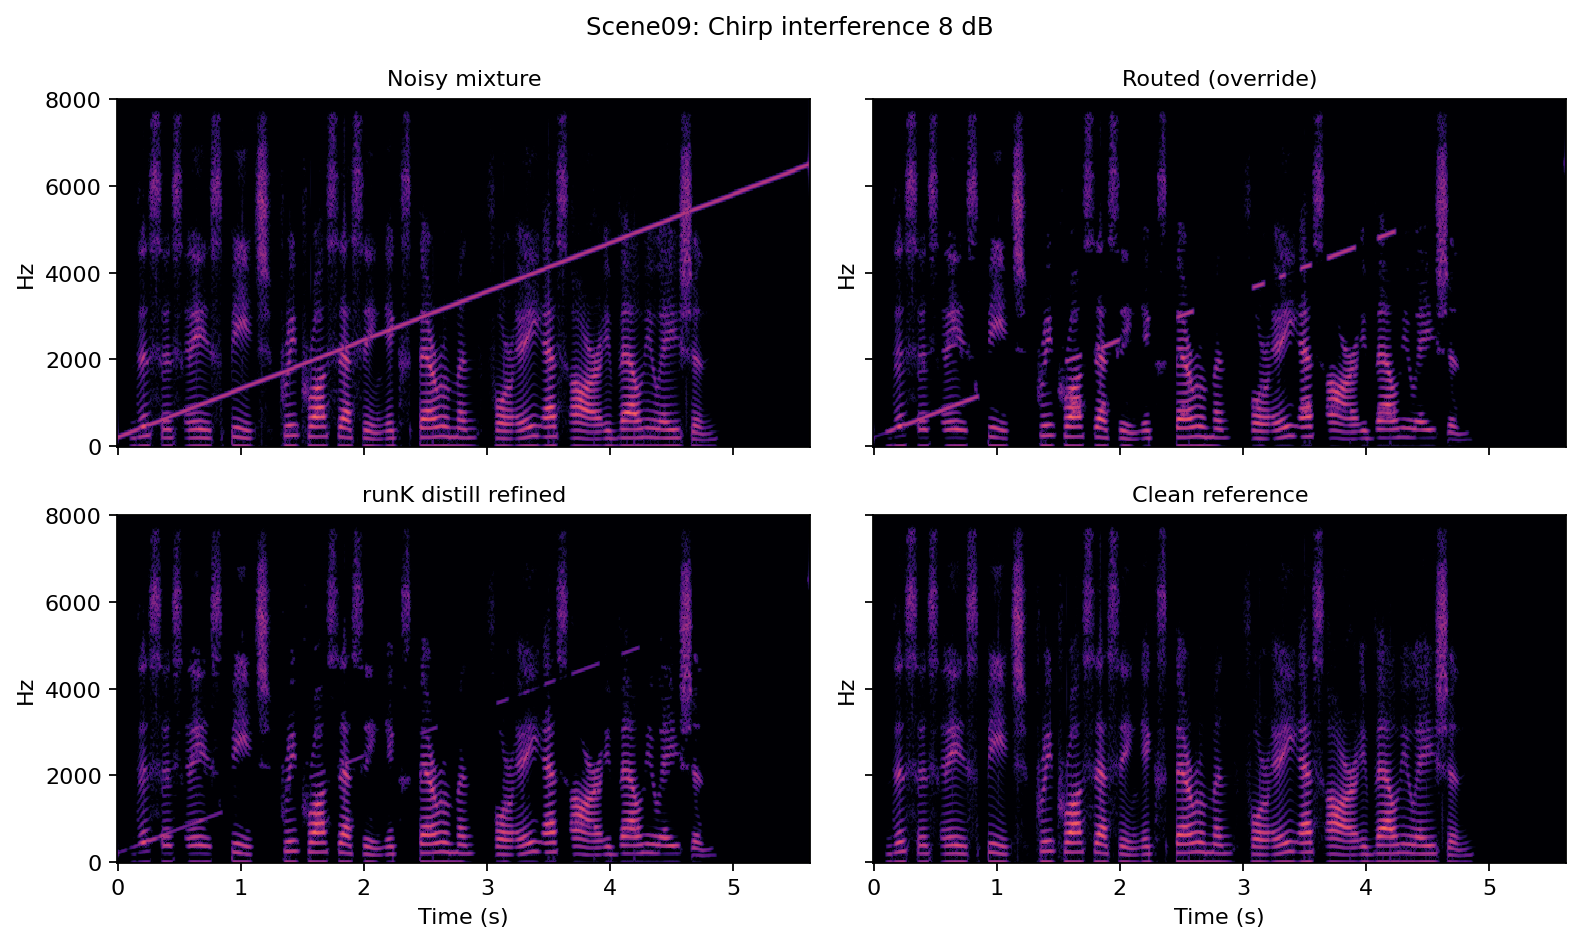
\includegraphics[width=0.95\textwidth]{figures/experiments/spectrogram_scene09_chirp_interference_snr8.png}
  \caption{Scene09 (chirp): runK refinement substantially reduces residual ridge energy vs.\ routed output alone.}
  \label{fig:spec_scene09}
\end{figure}

\begin{figure}[H]
  \centering
  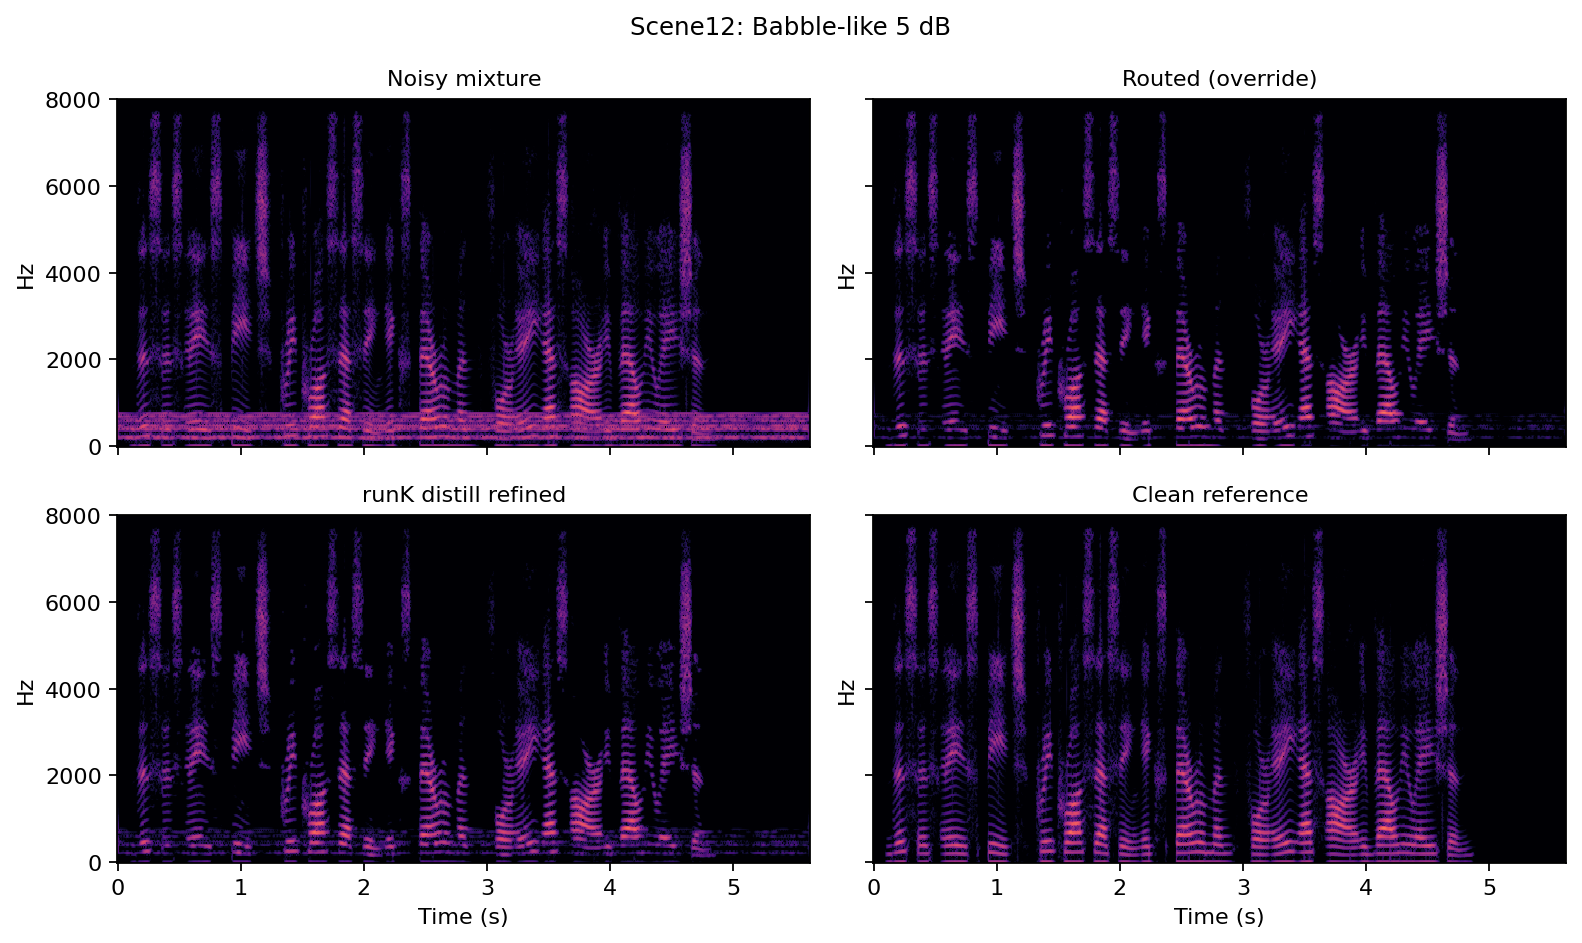
\includegraphics[width=0.95\textwidth]{figures/experiments/spectrogram_scene12_babble_like_snr5.png}
  \caption{Scene12 (babble-like): WPE routing + runK refinement recover clearer mid-frequency formants.}
  \label{fig:spec_scene12}
\end{figure}

\begin{figure}[H]
  \centering
  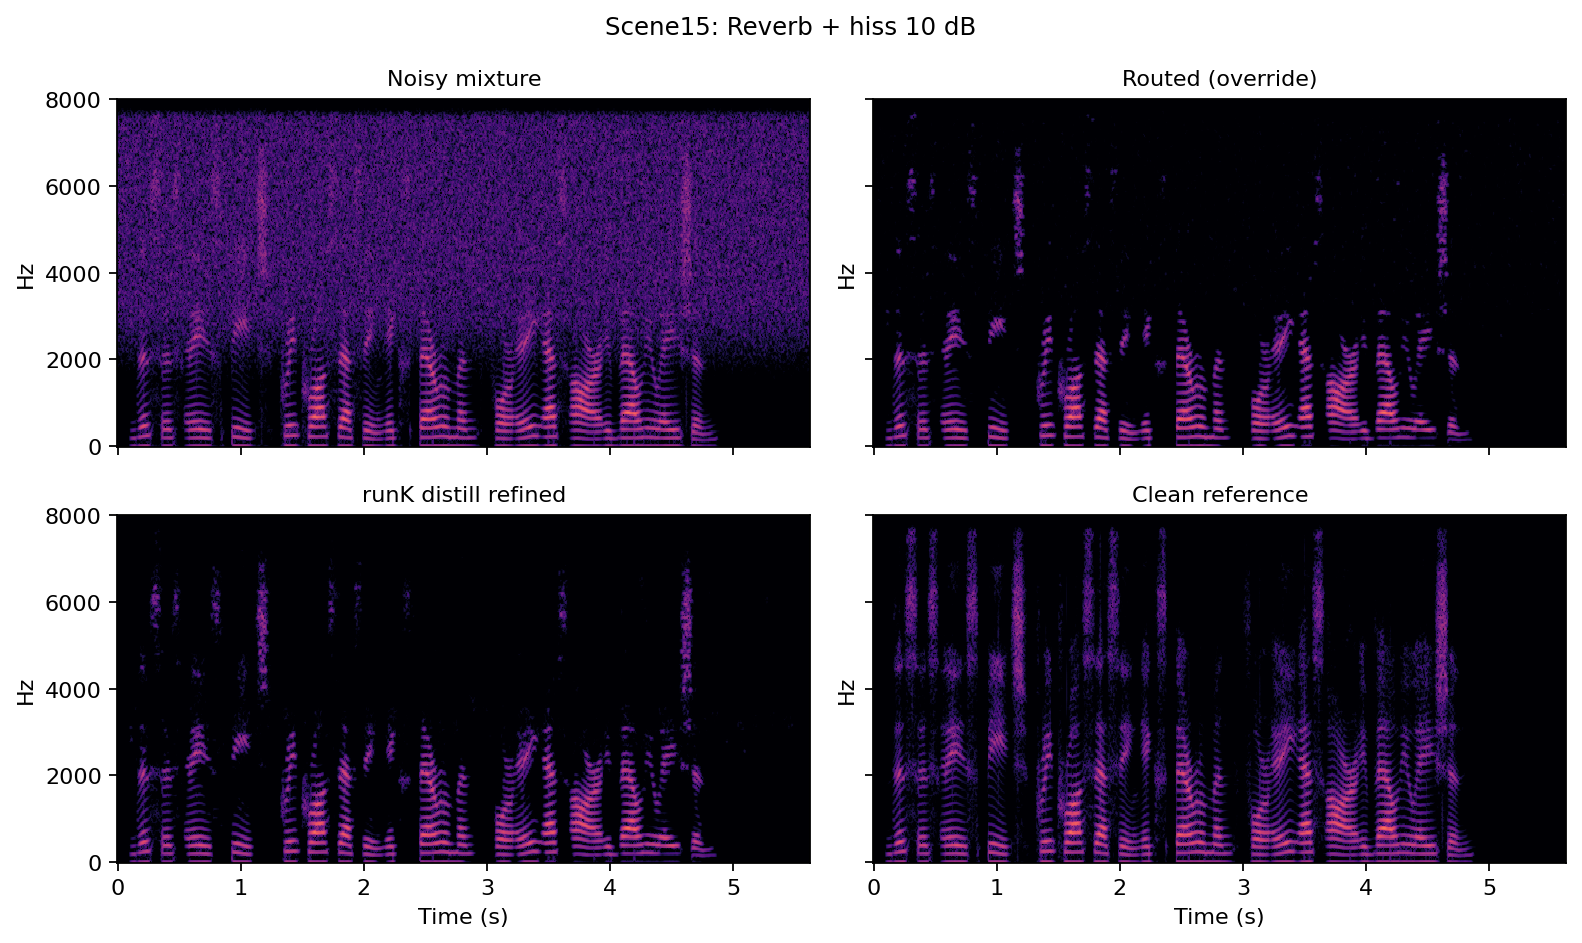
\includegraphics[width=0.95\textwidth]{figures/experiments/spectrogram_scene15_reverb_plus_hiss_snr10.png}
  \caption{Scene15 (reverb + hiss): runK refined output aligns more closely with clean reference timing.}
  \label{fig:spec_scene15}
\end{figure}

\section{Runtime Analysis}
\label{sec:runtime}

\begin{table}[H]
  \centering
  \caption{Measured processing latency (CPU, 5.6\,s clip).}
  \label{tab:runtime}
  \begin{tabular}{lcc}
    \toprule
    \textbf{Stage} & \textbf{Latency} & \textbf{Notes} \\
    \midrule
    \texttt{base\_omlsa\_mcra}     & $\approx 93$\,ms   & Single pass, 16\,kHz \\
    TinyResidualRefiner runK     & $\approx 8$\,ms    & STFT + dilated Conv + iSTFT \\
    Full hybrid (route + refine) & $\approx 100$--200\,ms & Depends on override module \\
    DeepFilterNet3 CLI           & $\approx 2.9$\,s   & dfnet311 Python CLI \\
    Student training (\texttt{runK}) & 1200\,s & 21\,488 steps, offline \\
    Teacher generation (15 scenes) & $\approx 44$\,s & offline batch \\
    \bottomrule
  \end{tabular}
\end{table}

\section{Discussion of Results}
\label{sec:exp_discussion}

\paragraph{RQ: Lightweight distillation.}
runK yields uniform incremental improvement (15/15 scenes) without RMS regressions vs.\ routed output, validating Proposition~\ref{prop:distill_improve}. Mean $\Delta$RMS ($1.39\times10^{-3}$) is more than double the legacy shallow \texttt{runD} student, with largest gains on structured interference (chirp, bursts).

\paragraph{RQ: Deployment trade-off.}
At 56\,129 parameters and $\approx 8$\,ms refine latency, runK occupies a favorable quality--cost point between routed math and DeepFilterNet3 teacher.

\section{Chapter Summary}
\label{sec:exp_summary}

On the 15-scene benchmark, override routing achieves mean RMS $0.00837$ (vs.\ $0.00936$ base OM-LSA), runK refinement further reduces mean RMS to $0.00730$ with improvements on every scene, and DeepFilterNet3 teacher reaches $0.00596$ at much higher inference cost. Mean SNR progresses from 9.07\,dB (noisy) to 14.06\,dB (runK) vs.\ 16.07\,dB (teacher). \chapref{ch:discussion} and \chapref{ch:conclusion} interpret these findings.
